\documentclass[10pt,a4paper]{article}
\usepackage{fontspec,polyglossia}
\setmainlanguage{russian}
\setmainfont{Times New Roman}
\usepackage{amsmath,amssymb,booktabs,tabularx,graphicx}
\usepackage[margin=17mm]{geometry}
\usepackage[hidelinks]{hyperref}
\usepackage{titlesec}
\titleformat{\section}{\large\bfseries}{}{0pt}{}
\titlespacing*{\section}{0pt}{8pt}{4pt}
\setlength{\parindent}{0pt}
\setlength{\parskip}{4pt}
\setlength{\emergencystretch}{3em}
\begin{document}
{\Large\bfseries Обучение рекуррентной сети циклическому движению: проверка MG}\par\medskip

29 сентября 2026 года. Выполненный эксперимент; CPU, без Colab.

\textbf{Результат.} В пяти исходно хаотических сетях обучение сформировало почти периодическое движение. MG по одному заранее выбранному нейрону снизился с 3.56--5.07 до 1.08--1.13. Снижение воспроизвелось для всех трёх наблюдаемых нейронов и всех проверенных окон и задержек. Полный спектр Ляпунова независимо подтверждает исчезновение заметных положительных показателей. Строгий заранее заданный критерий устойчивого цикла прошли 4 из 5 сетей; пятая имеет слабое поперечное сжатие. Это более устойчивый положительный пример, чем предыдущий опыт с neural collapse, но пока на небольшой модельной задаче.

\section*{1. Что учится и зачем}

Рекуррентная сеть учится \textbf{сама генерировать две согласованные периодические команды}, описывающие восьмёрку. Такие генераторы могут использоваться как блоки ритмического управления или воспроизведения сигналов. Здесь проверяется только генератор: робота, физической среды и реального датасета нет. Это прикладной прототип, а не демонстрация на LLM/CV.

Вначале рекуррентные связи случайны, выходные веса нулевые. Обучаем выходные веса методом рекурсивных наименьших квадратов (FORCE); выход возвращается в сеть, поэтому обучение меняет её автономную динамику. \textbf{Во время проверки веса заморожены, целевой сигнал в сеть не подаётся.} Измеряем самостоятельное движение сети после разных этапов обучения, а не временной ряд loss оптимизатора.

Состояние сети $x_t\in\mathbb R^{256}$, активности $r_t=\tanh x_t$, выход $z_t=W^Tr_t\in\mathbb R^2$. Один шаг модели:

\[
x_{t+1}=(1-h)x_t+h(J+UW^T)\tanh x_t,\qquad h=0.1.
\]

$J$ --- фиксированная матрица $256\times256$, $U$ --- фиксированная обратная связь $256\times2$, $W$ --- обучаемые 512 весов. Элементы $J$ независимы и распределены как $\mathcal N(0,1.5^2/256)$, элементы $U$ равномерны на $[-1,1]$, $x_0\sim\mathcal N(0,0.5^2I)$, $W_0=0$. Время релаксации равно 1. Целевые команды при физическом времени $s$:

\[
f(s)=\left(\sin\frac{2\pi s}{T},\;\frac12\sin\frac{4\pi s}{T}\right),\qquad T=10\pi.
\]

Каждые два шага после обновления состояния вычисляем $e=W^Tr-f(s)$, $v=Pr$, $a=1+r^Tv$, затем одновременно $W\leftarrow W-ve^T/a$, $P\leftarrow P-vv^T/a$; $P_0=I$. Всего 40 000 шагов модели, то есть 20 000 обновлений RLS. Ни число нейронов, ни ранг параметризации искусственно не уменьшаются. Цель входит только в ошибку обучения, не в уравнение движения.

\section*{2. Какие запуски сравниваются}

Настройки выбраны по задаче и независимой динамике на pilot seed 0, \textbf{до вычисления MG}. Неудачные пилоты сохранены: при 128 нейронах исходная сеть сама затухала; при 256 и усилении 1.8 обучение не давало нужного движения. Зафиксировано 256 нейронов и усиление 1.5.

Сначала выполнены все seeds 1--5 без отбора: все выучили движение, но лишь часть была хаотической до обучения. Поэтому добавлена отдельная группа для конкретного вопроса «обучение из хаоса к циклу»: из seeds 6--30 по порядку приняты первые пять с положительным старшим показателем более 0.01 и на всей записи, и на её второй половине. Проверены 13 кандидатов, приняты \textbf{7, 9, 15, 16, 18}. Отбор использует только необученную сеть, 16 384 шага после 2000 шагов разгона; MG при отборе не вычислялся. После обучения никто не исключён. Итоги этой группы условны на исходно хаотическую динамику, не являются долей успеха среди всех случайных сетей.

\newpage

\section*{3. Что и как измеряется}

Сохраняем веса на шагах 0, 2000, 8000, 20 000, 40 000. Для каждого снимка запускаем автономную сеть из её текущего состояния; отбрасываем 2000 шагов, затем записываем 8192 последовательных состояния, примерно 26 периодов целевого движения. Проверка не меняет последующее обучение.

\textbf{Независимая проверка.} На шагах 0, 8000 и 40 000 вычисляем все 256 конечновременных показателей Ляпунова. Якобиан именно дискретной модели:

\[
D F(x)=(1-h)I+h(J+UW^T)\operatorname{diag}(1-\tanh^2x).
\]

Случайный ортонормированный базис переносится каждым Якобианом; QR выполняется каждые 10 шагов. Первые 1000 шагов переноса отбрасываются, суммы логарифмов диагонали $R$ делятся на физическое время оставшихся 7190 шагов. Сохраняется также оценка по первой половине для проверки чувствительности к длине записи. Якобиан проверен конечными разностями, относительная ошибка менее $10^{-8}$. Это численная конечновременная проверка, не доказательство асимптотической устойчивости.

Дополнительно ищем возврат \textbf{всего состояния} через период $p$ в диапазоне $[0.8T/h,1.2T/h]$ с линейной интерполяцией дробного сдвига:

\[
R_x=\min_p\sqrt{\frac{\langle\|x_{t+p}-x_t\|^2\rangle}
{\langle\|x_t-\bar x\|^2\rangle}}.
\]

Малый $R_x$ подтверждает повторение полного состояния с ожидаемым периодом. Это проверка известной целевой периодичности, а не универсальная мера сложности. Ошибка задания --- RMSE двух выходов, нормированная на $\sqrt{0.3125}$, с подбором единого фазового сдвига по сетке из 720 значений. Частота и масштаб времени не подбираются. Ошибка без фазового выравнивания также сохранена.

До MG задан строгий критерий конечного режима: NRMSE $<0.1$, $R_x<0.1$, $|\lambda_1|<0.005$, $\lambda_2<-0.005$. Наличие низкой ошибки задания исключает тривиальный ответ «сеть просто остановилась».

\textbf{MG.} Наблюдаем только $y_t=\tanh x_{t,0}$; дополнительно проверяем заранее выбранные нейроны 1 и 2. Для каждого --- два непересекающихся окна по 4096 отсчётов. Каждое окно стандартизуется, строятся задержанные векторы с $E=20$, задержкой $\tau=4$ шага и $k=20$ соседями. Соседи ближе 156 шагов по времени исключаются (Theiler). Использована существующая реализация pooled-оценки проекта, без изменения ядра. Итог в таблице --- медиана двух окон, не выбор лучшего.

Для проверки чувствительности повторяем при $E=40$ с тем же исключением; записываем $I=MG_{40}/MG_{20}$. Дополнительные настройки для нейрона 0: окна 2048 и 8192 при $\tau=4$; задержки 2 и 8 при окне 4096 (Theiler $=39\tau$). Везде $k=20$, dither $10^{-9}$ после стандартизации. Значение $I\approx1$ показывает лишь стабильность к удвоению вложения, не доказывает все условия теории.

\textbf{Дешёвые альтернативы.} На том же скалярном сигнале считаем стандартное отклонение, нормированную энтропию FFT-мощности и ошибку возврата около известного периода. Отдельно вычисляем только старший показатель Ляпунова одним касательным вектором. Сравнение с ними не позволяет приписать MG универсальное преимущество по скорости.

\newpage

\section*{4. Что получилось}

\begin{center}\small
\begin{tabularx}{\linewidth}{l>{\raggedright\arraybackslash}X>{\raggedright\arraybackslash}X>{\raggedright\arraybackslash}X>{\raggedright\arraybackslash}X}
\toprule
Seed & MG до / после & Старший показатель до / после & Второй после & NRMSE после \\
\midrule
7 & 5.07 / 1.13 & +0.0198 / -0.0004 & -0.0164 & 0.0016 \\
9 & 4.84 / 1.13 & +0.0392 / +0.0000 & -0.0022 & 0.0048 \\
15 & 3.95 / 1.08 & +0.0317 / +0.0003 & -0.0106 & 0.0093 \\
16 & 3.56 / 1.13 & +0.0284 / +0.0003 & -0.0139 & 0.0019 \\
18 & 4.85 / 1.08 & +0.0219 / +0.0004 & -0.0152 & 0.0012 \\
\bottomrule\end{tabularx}\end{center}

У всех пяти начальный старший показатель положителен, после обучения близок к нулю; остальные ведущие показатели уходят в отрицательную область. Ошибка полного возврата уменьшается с 0.85--1.57 до примерно $7.3\cdot10^{-5}$--$1.2\cdot10^{-4}$. Подобранный период после обучения --- 314.11--314.18 шага против целевого 314.159. Это независимо подтверждает почти периодическое движение, а не только падение скалярной оценки.

\textbf{Строгий критерий прошли 4/5.} Seed 9 имеет $\lambda_2=-0.00222$, что отрицательно, но слабее заранее заданного порога $-0.005$. Сеть оставлена в результатах. Нельзя писать, что во всех пяти доказан одинаково устойчивый цикл.

\begin{center}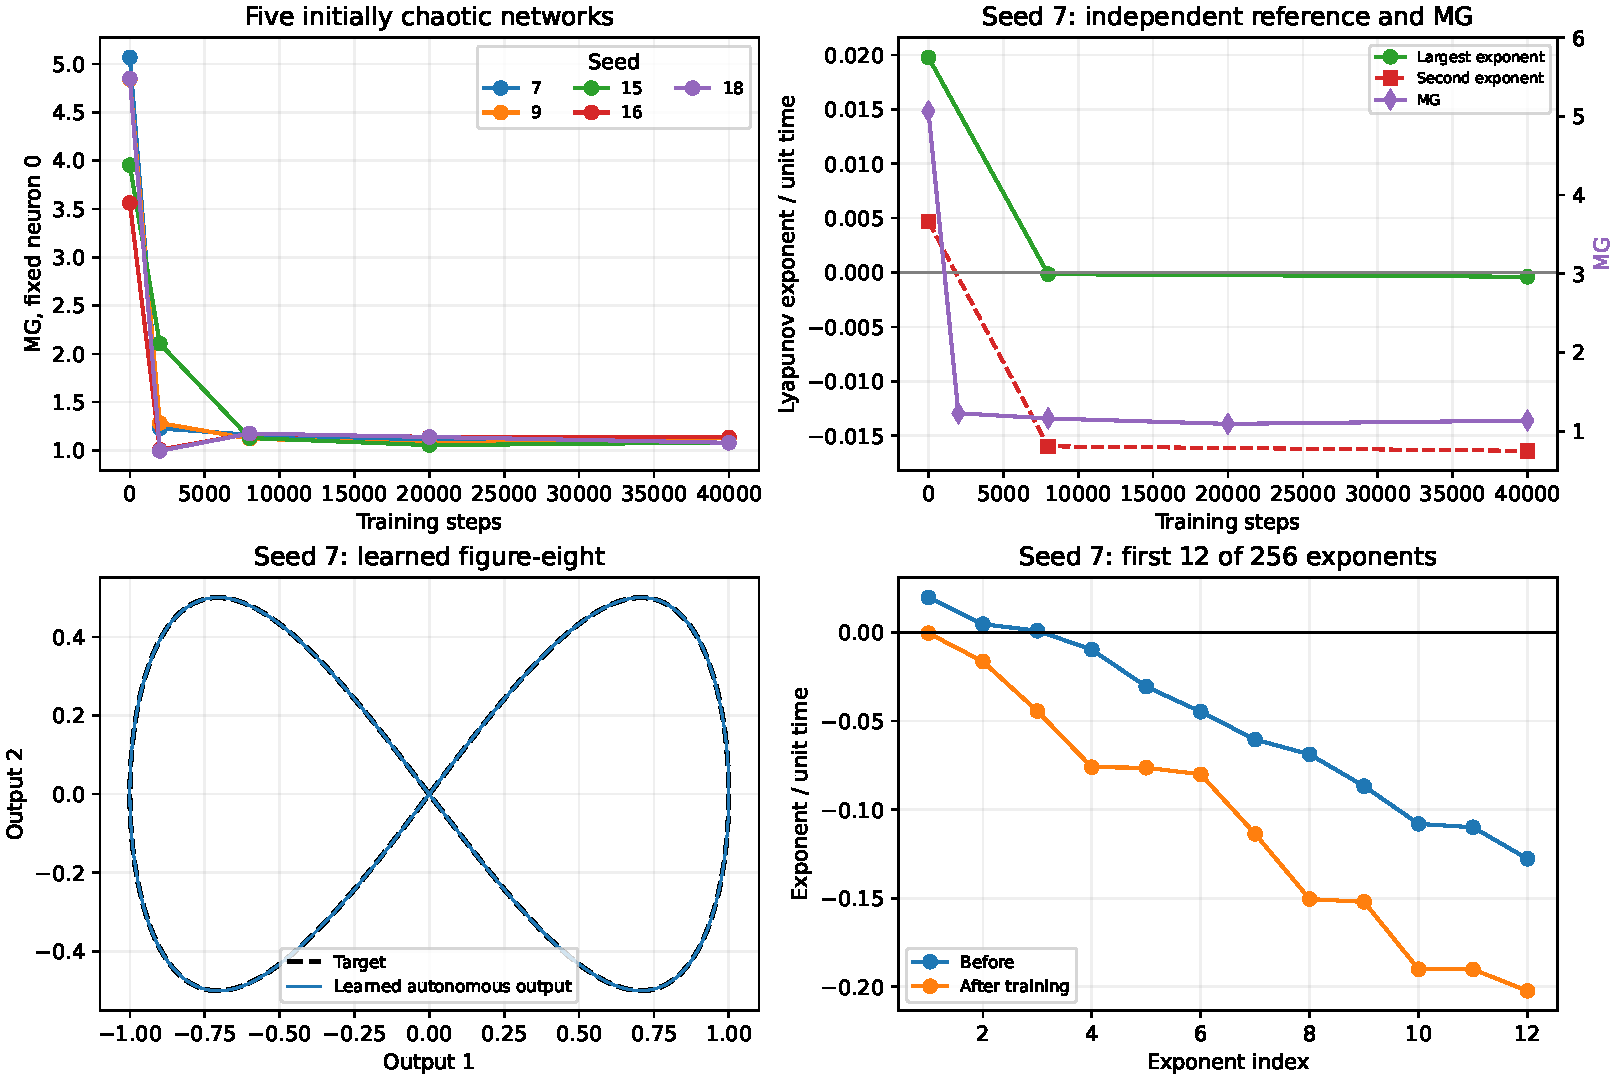
\includegraphics[width=\linewidth,height=.49\textheight,keepaspectratio]{results_chaotic/report_figure.pdf}\end{center}

На рисунке сверху слева --- все пять сетей; остальные панели относятся к одному seed 7, выбранному как первому принятому seed, без выбора по величине эффекта MG. Справа сверху MG и показатели Ляпунова вычислены по одним автономным записям. Линии между контрольными этапами только соединяют измерения.

\newpage

\section*{5. Насколько результат устойчив}

\textbf{Датчики и настройки.} MG снизился во всех 15 парах «5 сетей \ensuremath{\times} 3 фиксированных нейрона»: на 68--80\%. Для основного нейрона снижение составило 68--78\%. Все 20 дополнительных пар «seed \ensuremath{\times} настройка окна/задержки» сохранили направление эффекта. Это повторные измерения тех же пяти моделей, а не 35 независимых запусков. До обучения $I=1.18$--$1.57$, после --- $1.006$--$1.016$: исходные значения MG нельзя выдавать за точно восстановленное число компонент. После обучения оценка стабильнее и близка к единице.

\textbf{Это не просто уменьшение амплитуды.} У основного нейрона стандартное отклонение после обучения выросло в 4/5 сетей, тогда как MG снизился во всех. Умножение исходного скалярного ряда на 0.1 изменило MG менее чем на $1.4\cdot10^{-15}$. Обучение выходного слоя с отключённой обратной связью оставило скрытую траекторию побитово неизменной при одинаковом начальном состоянии: обучение само по себе не создаёт падение MG.

\textbf{Возмущение состояния.} Для каждой обученной сети выполнены три запуска из $x+0.5\xi$, $\xi\sim\mathcal N(0,I)$, с seeds 11/12/13; после 2000 шагов разгона записаны 4096 шагов. Низкую ошибку задания сохранили 13/15 запусков, одновременно NRMSE $<0.1$ и $R_x<0.1$ --- 12/15. MG находится в диапазоне 1.12--1.91. При seed 7 / perturbation 11 он равен 1.15 при NRMSE 0.89: сеть пришла к простому, но неверному движению. Следовательно, \textbf{MG измеряет упорядоченность динамики, а не правильность задачи}. В seed 9 после возмущений видна медленная релаксация, согласующаяся со слабым поперечным сжатием.

\textbf{Неудобные результаты также сохранены.} В первой группе без отбора (seeds 1--5) все сети выучили движение, но у seeds 1/2 исходный спектр уже согласуется с простой устойчивой динамикой, а seed 4 затухает к фиксированной точке. Тем не менее при основном окне у seed 4 MG падает с 18.45 до 1.09; исходное $I=2.08$ сигнализирует о нестабильности размерной интерпретации. У seed 1 MG до обучения меняется с 16.67 при окне 2048 до 1.02 при 8192. Эти случаи показывают, почему нельзя объявлять любое падение MG доказательством уменьшения размерности.

\section*{6. Время и объём наблюдений}

Ниже медианы трёх последовательных повторов на CPU Intel i5-12500H, один поток BLAS, float64, seed 7. Каждый метод обрабатывает одну и ту же запись из 8192 отсчётов; для MG это два окна по 4096, времена суммированы. Обучение, загрузка файлов и общий разгон не входят в время анализа. Ядра предварительно прогреты.

\begin{center}\small
\begin{tabularx}{\linewidth}{>{\raggedright\arraybackslash}Xrr}
\toprule
Диагностика, вся запись & До обучения, с & После обучения, с \\
\midrule
MG, E=20: два окна & 0.8353 & 0.5983 \\
MG + повтор при E=40 & 2.2333 & 1.2135 \\
Полный спектр: 256 показателей & 12.0058 & 11.5511 \\
Только старший показатель & 0.1976 & 0.1530 \\
Возврат полного состояния & 0.4809 & 0.2089 \\
Скалярные std, FFT-энтропия и возврат & 0.0009 & 0.0015 \\
\bottomrule\end{tabularx}\end{center}

\textbf{Скорость.} MG без повторного вложения быстрее полного спектра в 14.4 раза до обучения и 19.3 раза после; с проверкой E=40 --- в 5.4 и 9.5 раза. Проверка E=40 --- только один диагностический тест, не полная сертификация применимости. Старший показатель Ляпунова, возврат состояния и простые скалярные метрики здесь дешевле MG. Генерация и запись всей траектории занимают медианно 0.133/0.176 с до/после; генерация со скалярным логированием --- 0.102/0.166 с. При их добавлении преимущество перед полным спектром сохраняется. Одна скалярная запись занимает 64 KiB против 16 MiB полного состояния: в 256 раз меньше. Это объём сохранённого ряда, не пиковая память алгоритма MG. Времена повторов заметно колеблются; сырые значения сохранены, приведённые отношения не являются аппаратно-независимыми константами.

\newpage

\section*{7. Что можно утверждать в статье}

\textbf{Подтверждённый тезис:} при обучении автономной рекуррентной сети генерации циклического сигнала MG по одному скрытому нейрону воспроизводимо отмечает переход от хаотической к почти периодической динамике. Направление эффекта согласуется с независимым полным спектром Ляпунова и повторяемостью состояния; сохраняется при смене датчика, окна и задержки. Для этой записи анализ MG существенно дешевле полного спектра и требует наблюдать один канал вместо 256.

\textbf{Граница вывода:} эксперимент не показывает превосходства MG над всеми способами обнаружить периодичность. FFT-энтропия и скалярный возврат тоже отмечают переход и намного дешевле; старший показатель Ляпунова дешевле MG, но требует модели и её производной. У MG здесь полезна возможность работать по скалярной записи и сопоставлять геометрию движения, а не уникальность сигнала перехода. Падение не равно гарантированному улучшению качества модели и не даёт точного числа активных компонент в исходном режиме.

Это положительный пример именно \textbf{обучаемой динамической системы}, но пока небольшой синтетической задачи. Здесь нет эксперимента на крупной нейросети, измерения энергопотребления или подтверждения масштабирования на GPU. Результат стоит использовать как дополнительное прикладное подтверждение вместе с grokking, сохранив отдельные формулировки для теоретической размерности и эмпирического индикатора упрощения.

\section*{8. Как воспроизвести и где лежат данные}

Папка research\_force\_motion содержит неизменённое ядро MG через импорт из code/actdim и следующие скрипты. run.py обучает сеть и сохраняет автономные записи; screen.py повторяет независимый отбор и обучение дополнительной группы; analyze.py вычисляет спектр, MG, проверки и графики; benchmark.py повторяет замеры времени; make\_report.py и build\_report.py собирают этот отчёт. Точные команды и версии зависимостей приведены в README.md и environment.json.

В results/ --- все пять запусков без отбора. В results\_chaotic/ --- основная таблица independent\_reference.csv, mg.csv и mg\_summary.csv, все настройки sensitivity.csv, возмущения perturbations.csv, screening.csv с 13 кандидатами и benchmark.csv с каждым повтором времени. В подкаталогах seed сохраняются веса, полные траектории, полный спектр и его оценка по половине записи. В pilot/, pilot256/ и pilot256\_g15/ сохранены все пилоты, в том числе неудачные. PROTOCOL.md фиксирует порядок решений и критерии до MG.

Отдельный компактный архив force\_motion\_report\_and\_sources.zip содержит отчёт, исходники, копию ядра MG, численные таблицы и графики. Крупные записи состояний и контрольные точки остаются в рабочей папке; их можно воспроизвести указанными командами. Статья и её шесть PDF этим экспериментом не изменялись.

Метод обучения: D. Sussillo, L. F. Abbott (2009), “Generating Coherent Patterns of Activity from Chaotic Neural Networks”, Neuron 63, 544--557, DOI: 10.1016/j.neuron.2009.07.018. Результаты и замеры в этом отчёте получены в текущем запуске; исходная статья FORCE не является источником приведённых чисел.
\end{document}